\chapter{Metering and Billing of Energy on Ethereum}\label{ch:implementation}

Smart contracts can transform the energy industry. In this chapter we explore the inefficiencies of the energy market and identify gaps which can be filled by blockchain. We go through the advantages of an energy-based application built on smart contracts. Finally, we describe the business logic of a specific energy use-case which we implemented on Ethereum. The implementation takes into account the methods and concepts described in Chapter \ref{ch:scalability} and Chapter \ref{ch:security} in order to ensure that the smart contracts are efficient and robust.


\section{Energy Market inefficiencies}

The global energy market is gradually transitioning to clean and renewable energy. Regulations encourage usage of distributed energy resources (DERs) \cite{europe2030}. With the integration of DERs, consumers are gradually transforming to \textit{prosumers} who store their energy surplus or sell it to their peers, effectively distributing the generation of energy, contrary to existing power systems which were designed to accommodate central points of energy generation.

There are numerous inefficiencies which need to be resolved in today's energy markets~\cite{ey-inefficiencies}:
\begin{enumerate}
    \item \textbf{Transaction complexity:} More participants in the networks result in more complex transactions.
    \item \textbf{Predictability and Reliability:} Availability of DERs is less predictable compared to traditional energy resources like coal. 
    \item \textbf{Empowered prosumer:} There need be monitoring tools and infrastructure that allow prosumers to manage their energy production and consumption.
    \item \textbf{Geographic mismatches:} Locations that fully utilize DERs are usually far from key points of energy demand. Transmitting energy over long distances is inefficient.
    \item \textbf{Trust and Security:} New participants will only choose the system if it is able to be trusted and is properly secured.
\end{enumerate}

%Today's energy markets are called to resolve a number of issues.
% Having discussed how Ethereum works, and explained techniques to improve smart contracts' scalability and security, we proceed to discuss the topic of making energy markets more transparent and efficient by utilizing smart contracts. The use-case we describe can be used as a starting point for better tracking of energy usage inside a company, allowing better prediction of future needs.  
% The world is gradually shifting from nuclear and fossil fuels to Renewable Energy Sources (RES). RES have been taking a larger share of Germany's gross energy production and this has created a 
% Germany is on a rollout plan of installing smart meters in every household which incorporates RES.  
% The barrier to entry to become an energy producer\footnote{By installing solar panels for example} 
% Chart for renewables: https://www.cleanenergywire.org/factsheets/germanys-energy-consumption-and-power-mix-charts
% In its current state, most consumers do not know what they are paying Business level take long time and are 

% Price of energy, consumer does not know always what they pay, or what they gain from their renewables
 
\section{Energy Market use-cases for Blockchain}

A number of use-cases for smart contracts have been identified in the energy market. We proceed to describe applications that derive from the advantages of blockchain (transparency, trustlessness, security) as discussed in Section~\ref{advantages}.

\begin{enumerate}
    \item \textbf{Supply chain tracking and optimization:} This is a broad blockchain use case which allows for optimization on logistics and tracking the location of products, reducing fraud and ensuring the validity of an event.
    \item \textbf{Energy metering and billing:} By committing the values of energy consumed by entities to a blockchain, a timestamped record of meter readings gets generated which allows for the verification and more clear understanding of energy consumption across resources. This can be augmented to provide billing functionality (further described in \ref{business-logic}).
    \item \textbf{Peer to Peer (P2P) energy trading:} Consumers and prosumers operate in a local microgrid and trade energy between them, without a centralized operator, resulting in reduced loss of energy during transportation.
    \item \textbf{P2P Energy Micropayments:} A car that is far from its charging station is charged by the surplus energy of another car. Since this is a short-lived process that happens often, such as during the waiting time at a traffic light, in order to send and receive micropayments between the involved parties, a blockchain can be used to utilize fast payments and low transaction fees. 
    % It can also contribute to peak shaving~\footnote{Energy is billed based on the peak energy consumed during a time window. By consuming energy for charging during low peak times the peak can be reduced.} effectively reducing the costs during that time window.
\end{enumerate}

% By using smart contracts, all of the above use-cases can be automated
% Use Cases:
% - P2P Energy Trading
% - Sharing Economy - EV share and charge

% Internet of Things sensors can securely streamline inspections and repairs and automatically reduce outages.
% Applications have been developed \cite{DBLP:journals/ife/MengelkampNBDW18}

% Blockchains have the ability to provide transparency and immutability. Also,  When talking about energy and transparency, full history of meter readings, price calculation, billing of inhouse energy departments. This can be extended for EV car payment microtransactions and so on.

% The blockchain is a particularly interesting technology for decentralized processes that require large networks and trust relationships between all parties. Therefore, it offers great benefits to the power & utilities market, with its large networks of power and utilities companies, (maintenance) subtractors, (local) suppliers and end users.

% Smart meters Still, there are other applications that are ready for use in the near future. Smart meters for instance have already entered many homes. Up until now, sharing data through smart meters was a threat to the privacy of the owner of the meter. Again, the blockchain offers a potential solution. It can provide the accurate data to the supplier without requiring a direct link to the meter of specific users. When needed, the owner of the smart meter can prove to the supplier that the data are his, using his private key, and the cryptographic security of the blockchain proves that the information is accurate and hasn’t been tampered with. This puts the owner in control of his own data.

\section{Business Logic} \label{business-logic}
In collaboration with Honda R\&D Germany, we create a pilot suite of smart contracts for in-house use in order to track and bill the consumed energy of the company's headquarters as measured by a set of smart meters. 

We proceed to discuss the business logic of the use-case and then implement it. We utilize the Method 3 from Section \ref{method3} to optimize our smart contracts for gas efficiency, and utilize Slither from Section~\ref{slither} and the learned best-practices to ensure that the developed smart contracts are robust. The contracts were tested and deployed on a private Ethereum blockchain, however it is possible to deploy the implementation to the Ethereum mainnet.

%The purpose is to serve as a means of tracking the energy consumed by the company's smart meters and ensuring the data's validity and existence in a smart contract. In addition, due to the complex structure of the company, every smart meter's consumption can contribute with different coefficients to the total energy consumption of the rooms in a building. As a result, the developed smart contract are able to track the energy consumption of each room and assign it to a higher-order 

\subsection{Metering of Energy} \label{metering}

\paragraph{Smart Meters}

A smart meter is an energy meter which logs its measured energy readings to a monitoring server. A smart contract must track each smart meter by a unique identifier and store its power readings, along with the corresponding time of measurement. Due to the meter not being able to \textit{ping}\footnote{Hereafter, refers to a kWh,timestamp tuple which gets stored in the blockchain.} its reading directly to the blockchain, we create a pipeline where the reading and timestamp of each meter is pulled from the monitoring server and then pushed to the blockchain. 

\begin{figure}[ht!]
    \centering
    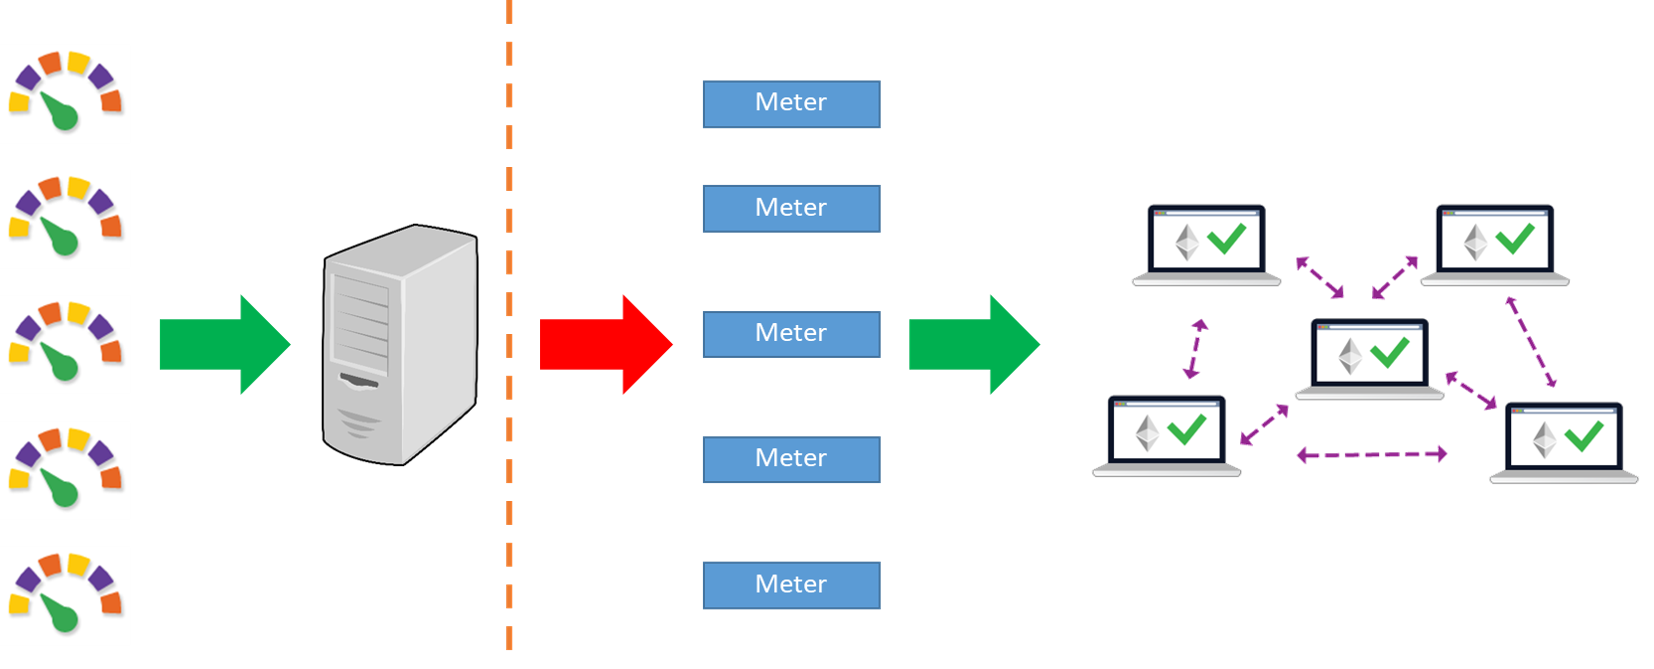
\includegraphics[width=\textwidth]{pull_push_monitoringserver}
    \caption{Meter Data gets pushed to the blockchain after getting pulled from the monitoring server}
    \label{fig:pull_push_monitoringserver}
\end{figure}
% must be able to keep track of the current reading and timestamp of the reading as well as the last reading and timestamp in order to calculate the difference of the two. It also has a unique identifier which is used to retrieve it in the smart contract.

\paragraph{Virtual Meters}

A \textit{Virtual Meter} is a group of \textit{Smart meters}. The purpose of a Virtual Meter (VM) is to track the consumption of multiple Smart Meters across various rooms of a company building. The consumption of a VM is a function of the power consumptions of its linked smart meters. 

The formula that describes each Virtual Meter is supplied from an internal partner and is considered to be known. An example formula can be seen in Equation \ref{eq:formula}. Variables prefixed with $VM$ represent Virtual Meters, $ELT$ and $KMZ$ represent Smart Meters and $F$ represent constants.

It is the case that this process could be done entirely on-chain, by creating a smart contract that manages virtual meters separately. This would require another smart contract for virtual meters, which would need to store the Meter IDs for each meter associated to the virtual meter, along with the formula that describes how the virtual meter consumption is calculated. This logic is unnecessarily complex to be performed on a smart contract directly. Instead, it is done off-chain on the client side, by pulling the readings of each smart meter, calculating the reading of the virtual meter, and then pushing the aggregated reading to the smart contract's storage.

\begin{equation} \label{eq:formula}
    \begin{aligned}
        VM15= \\
        & (ELT46-(ELT31+ELT16+ELT17+ELT35+ELT36))*F57
        \\
        + & (ELT35+ELT36-ELT18)*F27*F66
        \\
        + & (KMZ6-KMZ5)*(ELT16+ELT17+ELT18+ELT19+ELT20)\\
        & /KMZ2*F27*F66 
    \end{aligned}
\end{equation}

\begin{figure}[htb]
    \centering
    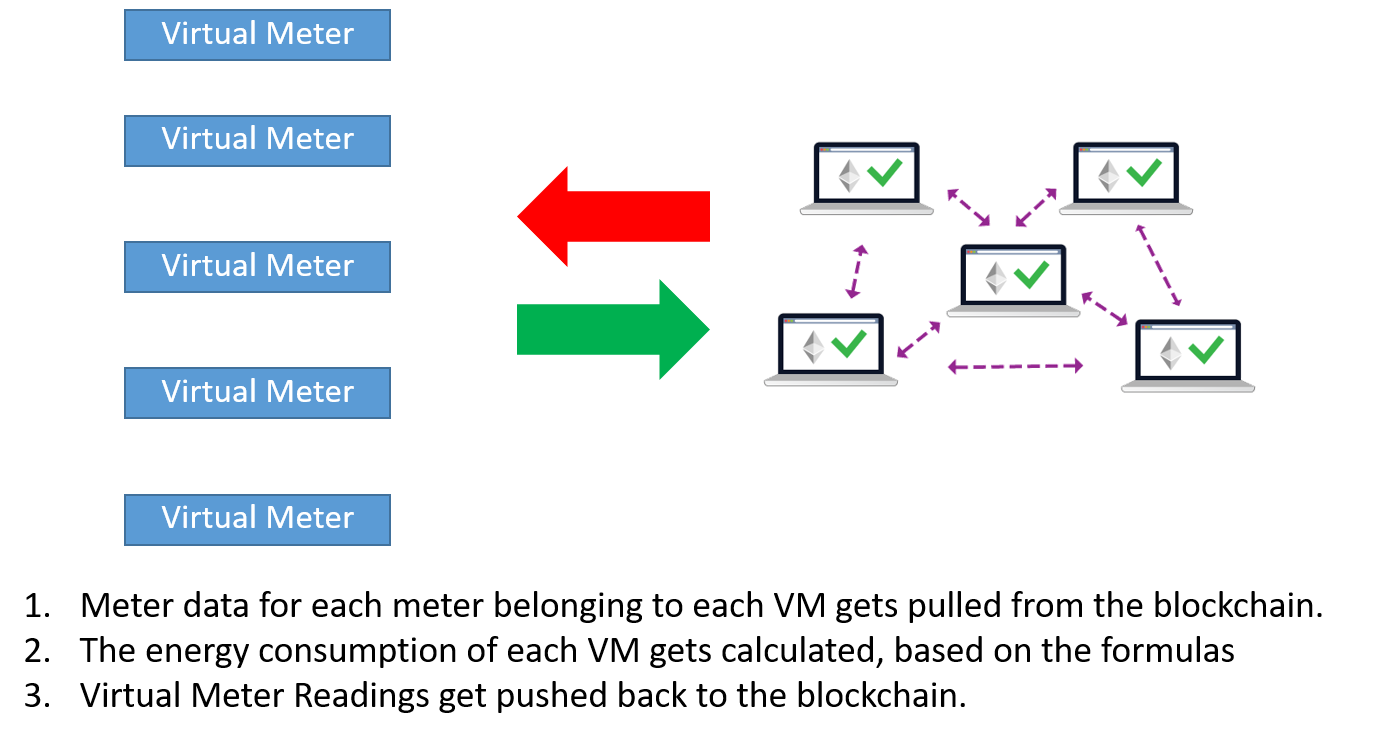
\includegraphics[width=\textwidth]{virtual_meters}
    \caption{The consumption of Virtual Meters gets calculated from the consumption of their associated Smart Meters.}
    \label{fig:virtual_meters_consumption}
\end{figure} % IMPROVE FIGURE

\subsection{Accounting Logic} \label{billing}

The accounting business logic of the company breaks down in a hierarchy which is described by \textit{Business Units} (BUs) and \textit{Departments}. BUs are used for external accounting, while Departments are used for internal accounting. In implementation terms, a Business Unit is equivalent to a Department.

A Department is composed of Virtual Meters, other Departments of a lower tier % better word?
 (hereafter called \textit{Subdepartments}) and \textit{Delegates}. A Department may forward its power consumption to its Delegates as part of the internal accounting process. The total consumption of a department is the sum of energy consumed by its Virtual Meters, Departments and Delegates. After a department delegates its debt, its consumption is considered to be cleared from an accounting perspective.

\begin{figure}[ht!]
    \centering
    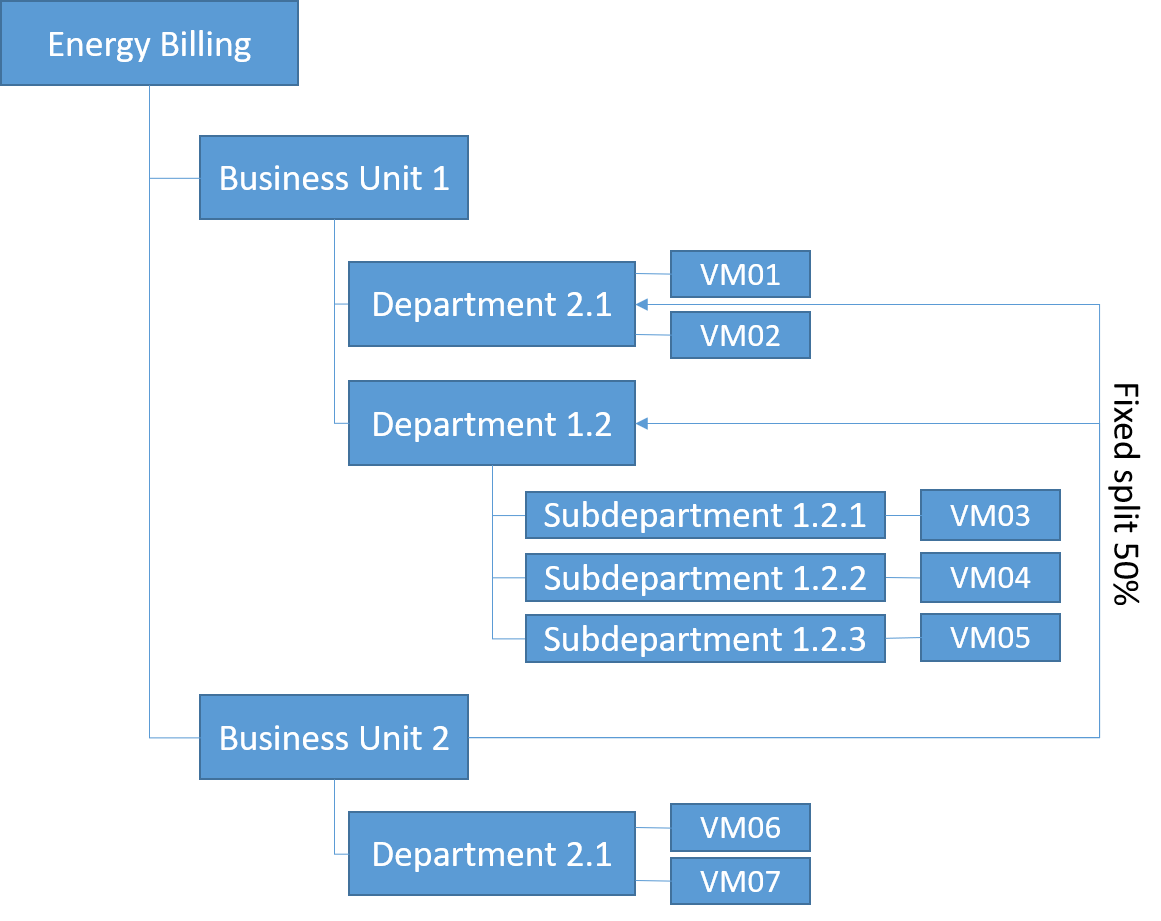
\includegraphics[width=.7\textwidth]{hierarchy}
    \caption{Relationship between Departments and Delegates.}
    \label{fig:hierarchy}
\end{figure} % TODO: BETTER FIGURE

There are two ways for a department to forward its consumption to its delegates:

\begin{enumerate}
    \item \textbf{Headcount Split:} Top tier departments can perform a headcount split of their consumption based on the percentage of staff that works at each \textit{Delegate} department.
    \item \textbf{Fixed Split:} This process can only involve a department which has exactly 2 \textit{Delegates}. The first delegate receives $X\%$ of the sender's consumption and the second delegates receives $(100-X)\%$.
\end{enumerate}

As an example, in \ref{fig:hierarchy} Department 1.1 and 1.2 are fixed split delegates of Business Unit 2. When BU2 forwards its consumption, it will get split among the 2 \textit{Delegates}. After delegation, Business Unit 2 has its consumption cleared and will not be calculated towards the total Energy Billing. The billing process starts from the inner-most tier and iteratively moves outwards until the top-tier departments are reached.


\section{Smart Contracts} \label{ch:implementation:sc}
In this section we go over the implementation and the rationale of each developed smart contract. We explain the inner workings and provide tests of their functionality. We follow the design principle that the data stored on the blockchain is the minimal amount of data that needs to be trustlessly verified. Any piece of data that can be derived from the already on-chain data is generated and verified off-chain. In case data does not need to be accessed by another contract but must be transmitted to an end-user, the \texttt{Event} functionality of Solidity is used (explained in \ref{apx:implementation:events}). 

\subsection{MeterDB}
MeterDB utilizes Method 3 (\ref{method3}) to keep track of the energy consumption values and logged timestamps of a smart meter or a virtual meter. We assume that a meter can be any IoT device that has its own Ethereum account\footnote{As a prerequisite, a private-public keypair needs to be generated for every meter.}. The contract is designed to map each Meter's address to its details (\texttt{id}, \texttt{reading}, \texttt{timestamp}).

The contract is split in two files, \texttt{MeterDB.sol} which contains the business logic, and \texttt{Meter.sol} which contains the gas optimization logic that encodes and decodes meter data in a \texttt{bytes32} variable. In order for a meter to be able to call the \texttt{ping} function it first needs to be activated, by registering its id and address in the smart contract. Deactivating a decommissioned meter results in its data being deleted from the storage of the smart contract, which refunds gas as mentioned in Rule 3 of \ref{ch:scalability}. By storing a mapping of meter ids to address we are able to access a meter's data by id in $O(1)$ instead of iterating over a list of registered meters.

For each meter, its latest reading is pulled from the monitoring server and if a new consumption value has arrived it replaces the previous reading along with its timestamp by calling \texttt{ping}. A \texttt{Pinged} event is emitted after each \texttt{ping} function call which enables users to fetch the full history of readings and timestamps for a meter. Table~\ref{table:meter} illustrates the design of the storage in \texttt{Meter.sol}.

\begin{table}[H]
	\centering
	\vspace*{-1ex}
	\scriptsize
	\vspace{-1ex}
	\caption{Required variables and size to describe a Meter.}
	\begin{tabular}{|c|c|c|}
        \hline
        \textbf{Name} & \textbf{Type}  & \textbf{Comment}\\ \hline 
        meterID      & bytes8         & IDs can be encoded in 8 bytes, can be optimized but hurts UX\\
        creationTime  & uint32         & Meter supports timestamps up to 2**32 = 02/07/2106 @ 6:28am (UTC) \\
        power         & uint32          & Power readings can reach up to 2**32, which is enough to store 1TWh readings \\
        \hline
    \end{tabular}
    \label{table:meter}
\end{table}

\subsection{AccountingDB}

AccountingDB stores the ids of each Virtual Meter, Subdepartment and Delegate in order to be able to calculate the consumption of each Department. 

The setting of energy reading values is done in \texttt{Department.sol} which utilizes Method 3 (\ref{method3}) to keep track of the energy consumed by a department due to its associated Virtual Meters, Subdepartments and Delegates. 

Due to the forwarding of a department consumption to another, we keep track of the power that is generated by the virtual meters, the delegated power that is received from another department, and the cleared power which is the amount of power that has been cleared from that department, either through delegation or from accounting. The consumption forwarding logic is implemented as described in Section~\ref{billing}. A \texttt{active} variable is used to keep track of activated departments.

\begin{table}[H]
	\centering
	\vspace*{-1ex}
	\scriptsize
	\vspace{-1ex}
	\caption{Required variables and size to describe a Meter.}
	\begin{tabular}{|c|c|c|}
        \hline
        \textbf{Name} & \textbf{Type}  & \textbf{Comment}\\ \hline 
        active         & bool         & Department active flag\\
        headcount      & uint7        & Headcount percentage, between 0 and 100\\
        power          & uint80       & Power readings can reach up to 2**80\\
        delegatedPower & uint80       & Power readings can reach up to 2**80\\
        clearedPower   & uint80       & Power readings can reach up to 2**80\\
        \hline
    \end{tabular}
    \label{table:department}
\end{table}

\subsection{Access Control} \label{acl}
As discussed in Chapter \ref{ch:security} enforcing proper access control on critical functions of a smart contract is very important. It is common to find Access Control Lists (ACL) in enterprise environments which allow only participants to access resources based on their clearance levels. This functionality does not exist by default in smart contracts. Access control can be done separately in each contract, by using a whitelist and a function modifier, however that needs to be done for each contract and does not scale for a rich smart contract ecosystem (further explained in \ref{apx:implementation:acl}). 

As a result, we use a pattern for access control by calling a separate smart contract that stores the logic for allowing or denying permission to a user about calling a function of a contract at an address. 

We proceed to describe the access control enforced on each of the actors involved in the developed smart contracts:
\begin{enumerate}
    \item Administrator: Can call all functions in all deployed contracts.
    \item Registry Operator: Can call \texttt{enable} and \texttt{disable} in \texttt{Registry}.
    \item Meter Operator: Can call \texttt{activateMeter} and \texttt{deactivateMeter} in \texttt{MeterDB}.
    \item Accounting Operator: Can call \texttt{activateDepartment}, \texttt{deactivateDepartment} \texttt{setDelegates},\texttt{setVirtualMeters},\texttt{setSubdepartments},   \texttt{setHeadcount}, in \texttt{AccountingDB}.
    \item Accountant: Can call \texttt{billPower}, \texttt{fixedSplit}, \texttt{headcountSplit} and \texttt{clearDepartment} in \texttt{AccountingDB}.
\end{enumerate}

\subsection{Contract Registry} 

In order to be able to retrieve the addresses of smart contracts by name a \texttt{Registry} smart contract was implemented. The contract resolves contract names to addresses through a \texttt{bytes32} to \texttt{address} mapping. The address of a contract can be changed by the registry's operator. This lays the foundation of a basic pattern for upgradeable smart contracts via a controlled name registry. Exploring the possible implementations of upgradeable contracts with this method is considered out of scope for this Thesis. Finally, this method can be utilized in the client scripts in Section \ref{ch:implementation:client} to reduce the number of addresses that need to be supplied to interact with the smart contracts\footnote{The registry's address is provided from the command line and then the registry resolves each contract's address by their names which are known beforehand}.

\subsection{Deployment Pipeline}

The full deployment pipeline involves deploying each contract separately and linking it to the Access Control List as shown in Figure~\ref{fig:pipeline}. At each step, the Administrator grants permissions to call specific functions of the smart contract to each role. Finally, after all contracts have been initialized, their addresses are stored in the Registry for later resolving.


\begin{figure}[htb]
    \centering
    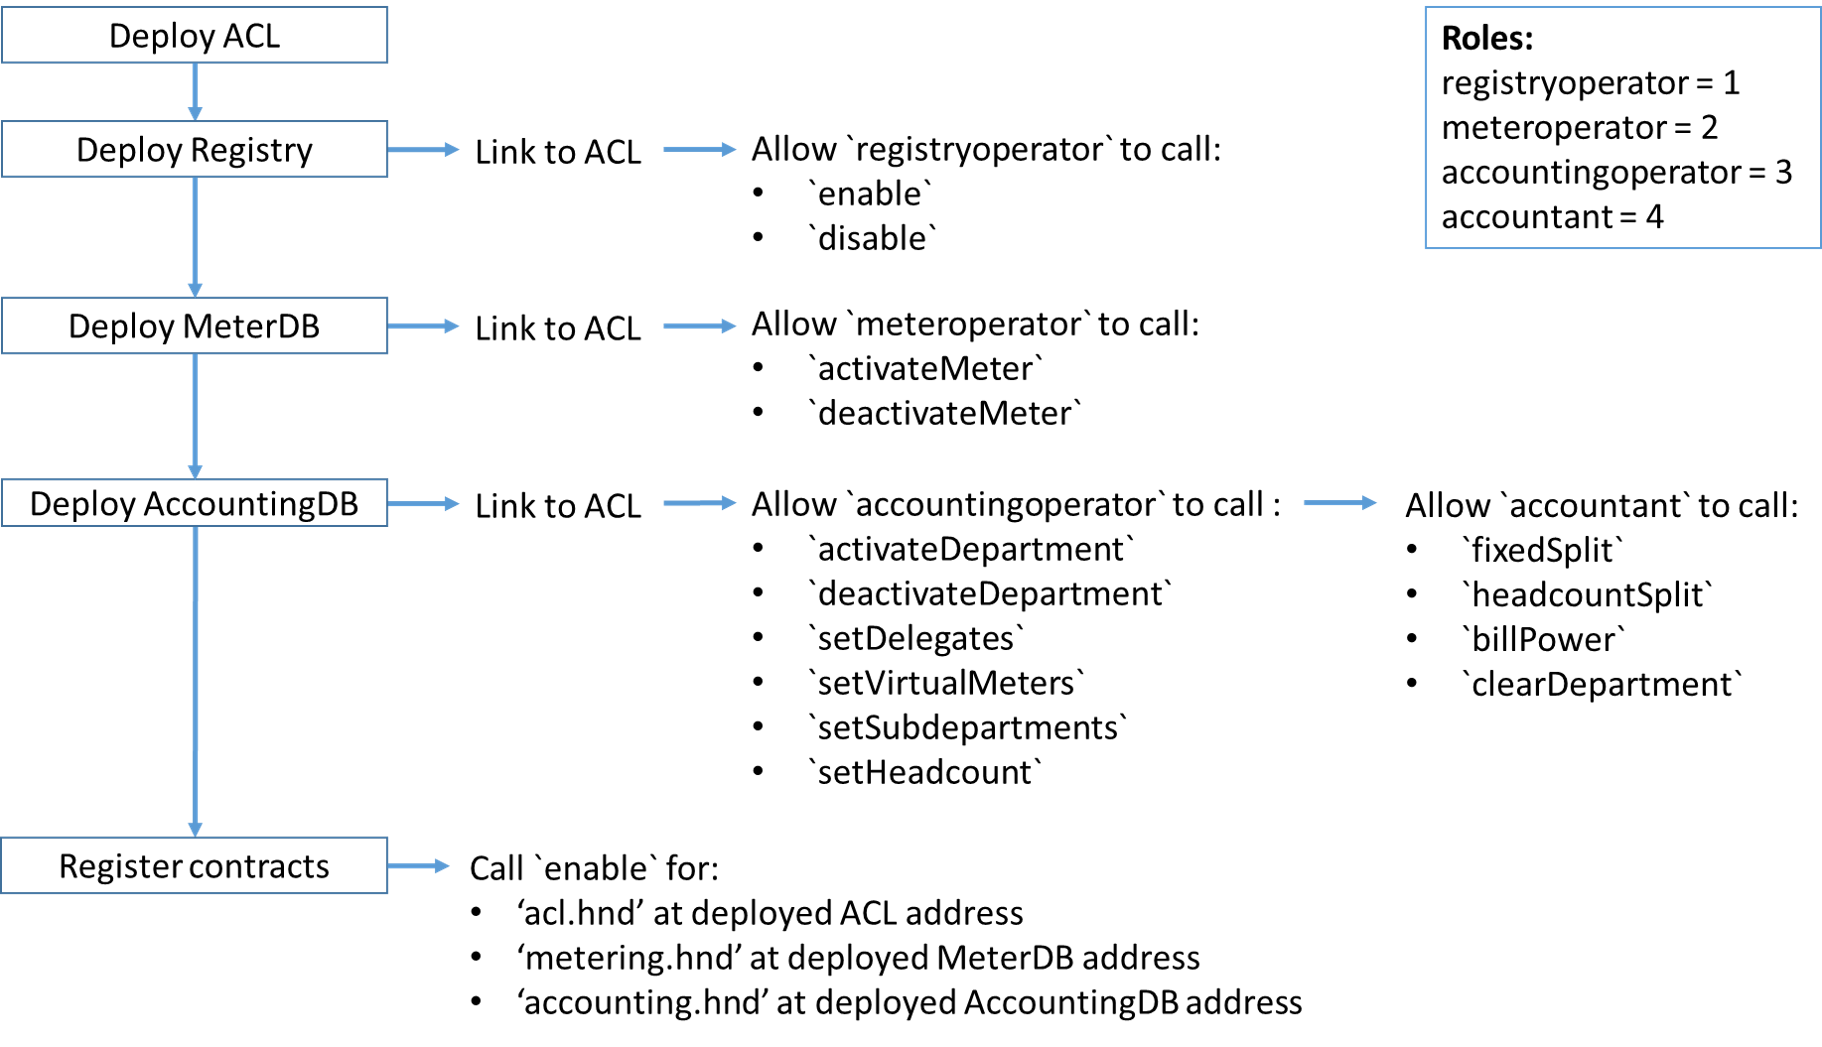
\includegraphics[width=\textwidth]{pipeline}
    \caption{The full deployment pipeline enforcing access control}
    \label{fig:pipeline}
\end{figure}

\section{Client Side} \label{ch:implementation:client}

As described in Section \ref{ch:basics:insideevm}, smart contract functions get executed only in response to transactions made by EOAs. Since the goal is to have an automated process of pulling data from and pushing data to the smart contracts, we implement client scripts which perform that functionality. We use Python and Web3.py to implement utilities and multiple command line interfaces (CLIs) which are used to interact with the smart contracts. A module is also developed for interacting with the REST API of the monitoring server. A separate keypair is generated for every role mentioned in Section \ref{acl}, and each CLI is designed to function only with by using the corresponding role's private key.

% In order to make the code portable and ensure that the clients can be run on any machine, we also provide a Dockerfile. Docker utilizes containerization Due to design, it can be dockerized and run on multiple blabla.

\subsection{Utilities} \label{utils}

\subsubsection*{Web3.py and Contract Wrappers}
We create a wrapper around the web3 library in order to provide a generic interface when connecting to a node. That way, a web3 instance can be return by calling \texttt{getWeb3(endpoint)}. In order to send a transaction, it first must be signed with the sender's private key. In the naive case, the private key can be stored in the node, however the security of this is limited to a user hosting their own node. In the case where multiple clients need to connect to a third-party node, it is a security compromise to host the unencrypted private keys on the node. 

We define a base class called \texttt{Contract} that provides functionality for interacting  with a smart contract. It allows signing and broadcasting of locally signed transactions to a node. It is able to track the nonces of an account separately which means that an account can submit multiple transactions without waiting for the previous one to get confirmed. It receives a compiled contract ABI and address of the corresponding contract, along with a private key for signing the transactions. The exposed function \texttt{sign\_and\_send} is used to specify which function of the contract to call and submit it for execution to an Ethereum node. We use the \texttt{Contract} class throughout our implementation to create user-friendly interfaces for the functions of each contract while maximizing code reusability and security by signing transactions locally.

\subsubsection*{Monitoring Server and Rest API}
As mentioned in Section \ref{metering}, there is no direct access to each meter's reading. As a result, all readings are exposed through an authenticated REST API. We implement a module which gets instantiated with a Meter id as a parameter, and is able to interact with the monitoring server API. The primary function used is \texttt{get\_single\_reading} which fetches 1 reading from the monitoring server, by default the most recent one. Implementing the whole set of functionality provided from the API was considered out of scope becaues it did not provide any additional information for our use-case.

\subsection{Administrator CLI}
The administrator role is used to grant or revoke role permissions to operators. The CLI interacts with the ACL smart contract which has been initialized as described in Section \ref{acl}.  As input, it expects an action (grant, revoke) and a json configuration file with the address of each account and its corresponding role to be granted or revoked. If no configuration file is supplied, it is expected that a role and address is provided as command line arguments. A user can additionally supply the \texttt{fund} parameter to send ether for the gas costs the operators will incur for interacting with their corresponding smart contracts. 

\subsection{Registry Operator CLI}
The registry operator's role is used to enable or disable a contract in the \texttt{Registry} contract. It can be utilized to register a new contract name and address at a later point in time or to remove an existing contract from the listing. The CLI also provides the functionality to resolve a contract name to its address or a contract address to its name. 

\subsection{Meter Operator CLI} \label{meter-operator}
The meter operator role is used to activate or deactivate smart meters in the \texttt{MeterDB} contract. The \texttt{ping} function is decorated with the \texttt{onlyMeter} modifier which requires for a meter to first be activated to successfully call it. As input, it expects a json configuration file with the address of each meter and its id. If no configuration file is supplied, it is expected that an address and a meter id is provided as command line arguments. By providing the \texttt{deactivate} parameter, it instead deactivates the meters. A user can additionally supply the \texttt{fund} parameter to send ether for the gas costs the meters will incur for calling \texttt{ping}.

\subsection{Accounting Operator CLI}
The accounting operator role is used to activate or deactivate departments in the \texttt{AccountingDB} contract. After activation, the operator should set the department's headcount, virtual meters, subdepartments and delegates according to the business logic. As input, the CLI expects a json configuration file which represents the business logic and which functions to be called for each department. 

\subsection{Single and Multiple Meters CLI}
A \texttt{meter} module is implemented which is responsible for connecting to \texttt{MeterDB} and the monitoring server through the API as explained in Section \ref{utils}. The meter first needs to be activated by the meter operator as explained in Section \ref{meter-operator}. The client is responsible for polling the monitoring server. When a new power reading arrives for the meter, it is pinged to the smart contract. The \texttt{single-meter} CLI expects the meter's private key as input, and retrieves the meter id from the smart contract in order to connect to the monitoring server.

Due to having multiple smart meters in our use-case, a \texttt{multiple-meters} CLI is also implemented which is responsible for launching multiple \texttt{single-meter} processes, each one running independently of each other. The output of each process is saved in a timestamped log file.

\subsection{Single and Multiple Virtual Meters CLI}
A \texttt{virtualMeter} module is implemented which is responsible for connecting to \texttt{MeterDB} and pulling the reading of its connected meters as described in Section \ref{metering}. Along with the virtual meter's private key a formula is supplied to the CLI as arguments. The virtual meter and the meters included in the formula must be previously activated by the meter operator. Given the formula, each referenced meter's readings are fetched, and the formula is evaluated\footnote{Using the module: \url{https://github.com/Axiacore/py-expression-eval}} before pinging the final value to the smart contract.

Similarly to normal smart meters, a \texttt{multiple-virtualmeters} CLI is implemented which is responsible for launching multiple \texttt{single-virtualmeter} processes, each one running independently of each other. The output of each process is saved in a timestamped log file.

\subsection{Accountant CLI}
The accountant module is responsible for pulling all the readings associated with a department, calculating the total amount of energy to be billed to the department as well as performing any forwarding of energy to a department's delegates. The accountant is simultaneously connecting to \texttt{MeterDB} and \texttt{AccountingDB}. Even though the accountant role is not authorized to access the functions related to pinging or operating in \texttt{MeterDB}, accessing the data for each meter can be done without supplying the contract instance with a private key\footnote{Viewing data stored in a smart contract is free as it involves directly querying the node for its storage and does not involve any state mutating transaction. As a result, no private key is needed to access the meter readings.} 

The departments are processed in order from the inner-most tiers towards the top level departments, as described in Section~\ref{billing}. The flowchart in Figure \ref{fig:consumption_flowchart} shows the process that each department goes through in order to correctly calculate its final consumption.
% since the consumption of a department may be dependent both on its associated virtual meters, which are stored in \texttt{MeterDB}, and its subdepartments or delegates. The connection 

\begin{figure}[H]
    \centering
    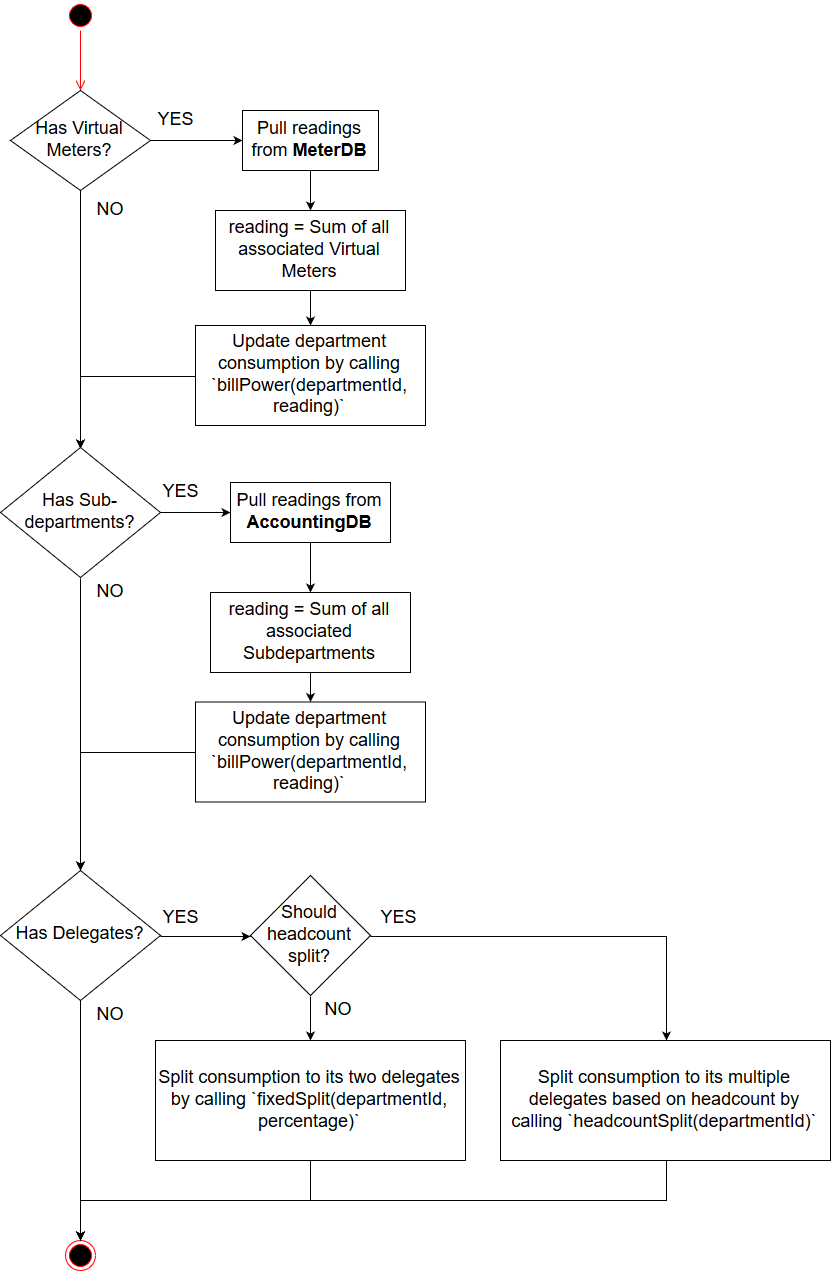
\includegraphics[width=\textwidth]{flowchart}
    \caption{Consumption calculation for a Department}
    \label{fig:consumption_flowchart}
\end{figure}

\subsection{Execution Pipeline} \label{execution}

Having described how each module of the client side works, in \ref{fig:execution} we show the order in which the client side programs get executed to provide the desired metering and billing functionality. Firstly, the administrator grants all of the needed privileges to the corresponding operators' addresses. The meter operator activates all meters, and all virtual meers. The accounting operator activates and initializes the accounting settings for each department. Each meter and virtual meter starts pushing their values asynchronously to the \texttt{MeterDB} contract, while at the same time the accountant is able to bill each department according to the logic which was previously specified by the accounting operator.

\begin{figure}[htb]
    \centering
    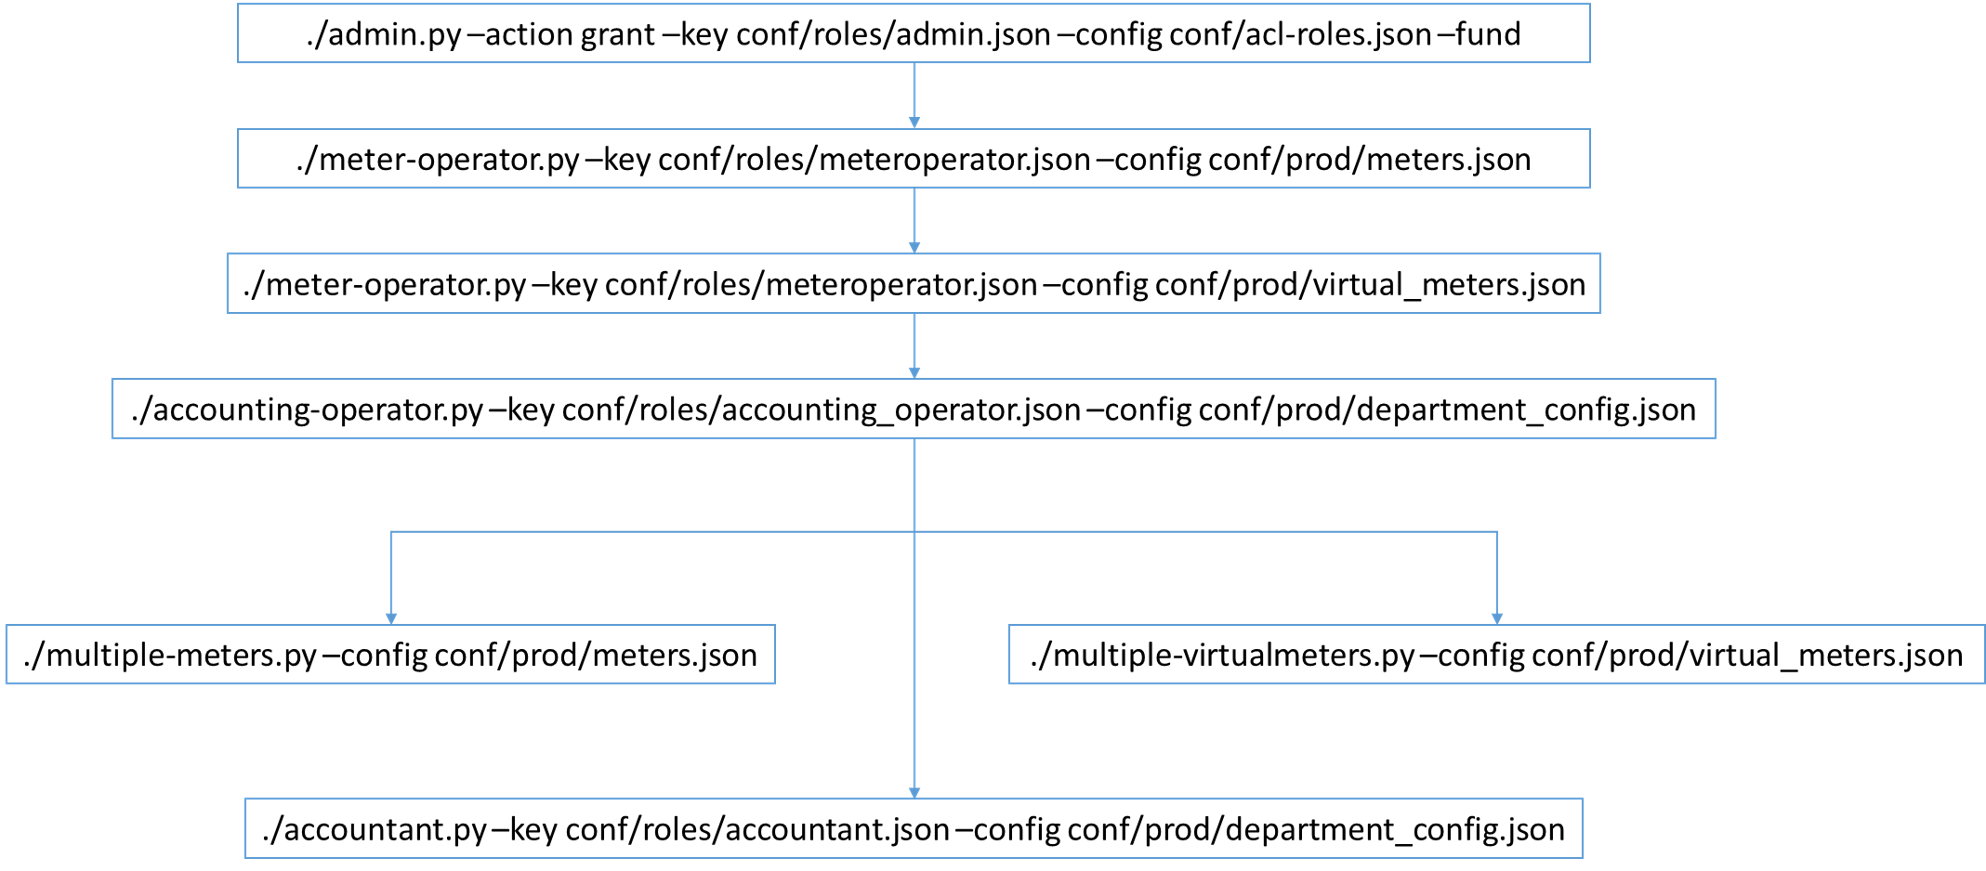
\includegraphics[width=\textwidth]{execution}
    \caption{The full execution process of metering and billing}
    \label{fig:execution}
\end{figure}
